% Created 2022-05-18 Wed 16:25
% Intended LaTeX compiler: pdflatex
\documentclass[a4paper, 11pt]{article}
\usepackage[utf8]{inputenc}
\usepackage[T1]{fontenc}
\usepackage{graphicx}
\usepackage{longtable}
\usepackage{wrapfig}
\usepackage{rotating}
\usepackage[normalem]{ulem}
\usepackage{amsmath}
\usepackage{amssymb}
\usepackage{capt-of}
\usepackage{hyperref}
\usepackage[margin=1.0in]{geometry}
\usepackage{amsmath}
\usepackage[nodisplayskipstretch]{setspace}
\author{Mick Harrigan}
\date{05/18/2022}
\title{\textbf{CMPE320 Project 5}\\\medskip
\large Map and ML Detection of Binary Signals}
\hypersetup{
 pdfauthor={Mick Harrigan},
 pdftitle={\textbf{CMPE320 Project 5}},
 pdfkeywords={},
 pdfsubject={},
 pdfcreator={Emacs 28.1 (Org mode 9.6)}, 
 pdflang={English}}
\begin{document}

\maketitle
\hrule

\setstretch{1.5}
\setlength{\parindent}{0pt}

\section{Introduction}
\label{sec:org9c63fbf}
This project investigates the autocorrelation of a random signal. The use of the MATLAB function \emph{xcorr} within the simulations allows the visualization of this random signal and its autocorrelation.

\section{Simulation and Discussion}
\label{sec:org37edc8d}
\subsection{Create a MATLAB Model}
\label{sec:org375a5aa}
The process for creating the model of random data and its autocorrelation is done across a few steps.
These steps are shown here below.

\begin{enumerate}
\item Generate random data for the time variable
\item Calculate the sample mean of the generated data
\item Calculate the autocorrelation of the data across different values of \(\tau\)
\item Calculate the sample mean of the autocorrelation across the same \(\tau\)
\end{enumerate}

These steps and their respective outputs are illustrated below in Figure \ref{fig:MatlabModel}.

\begin{figure}[htbp]
\centering
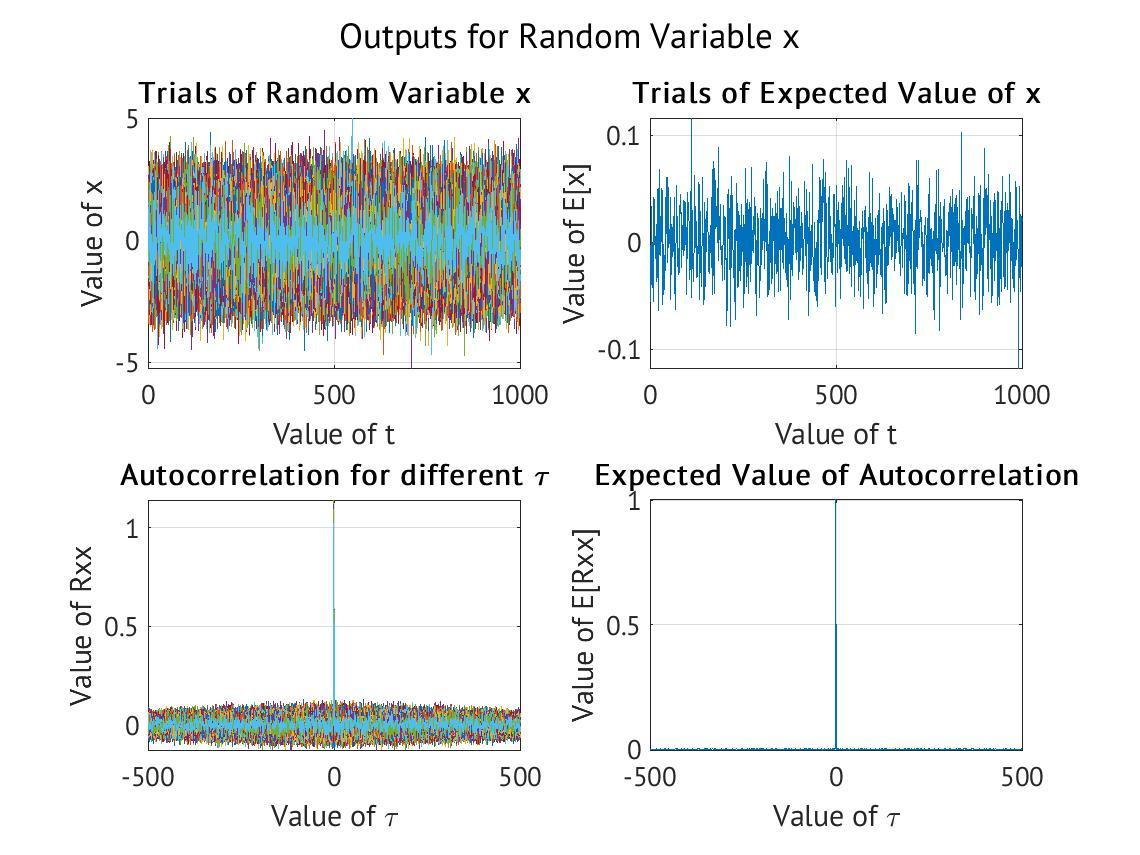
\includegraphics[width=.9\linewidth]{./Images/MatlabModel.jpg}
\caption{\label{fig:MatlabModel}Output of the 4 steps to find the autocorrelation of a random dataset}
\end{figure}

\pagebreak

Figure \ref{fig:MatlabModel} has 4 subfigures, where each graph is a step in the process to explain the autocorrelation of multiple random variables.
Subfigure 1 has the completely random generated data, and each trial is overlayed on top of every other trial.

Subfigure 2 has the expected value across time for all trials generated in the figure before. This is meant to be random as well, as the expected value of IID random variables is still random.

Subfigure 3 has the autocorrelation for different values of \(\tau\) and shows that the greatest autocorrelation is when \(\tau\) is closest to 0 meaning that the value of the random variables is closest the closer the time is to any other trial's output. In simpler terms, comparing trials at similar times (smaller values of \(\tau\)) has a much greater autocorrelation than that of different times (larger values of \(\tau\)).

Subfigure 4 has the sample mean of the autocorrelation, which effectively smooths out the randomness of the values with larger magnitudes of \(\tau\) and emphasizes when \(\tau\) is near 0 as that is when the values are most closely related (or the same).

The understanding that is taken from this is that the autocorrelation of these trials is generally random for any given \(\tau\), unless that \(\tau\) is 0 where the data being compared is itself. This is what leads to the spike at 0 and the randomness elsewhere. This spike is also the same as the variance of the random variable used in these trials.
This is equivalent to the data being white thus the true autocorrelation function is a delta function centered at \(\tau = 0\) which is what is found through each subfigure.

\subsection{Simulated Filtered Random Gaussian Data}
\label{sec:orgb3c6090}
This section differs from Section \ref{sec:org375a5aa} through the use of a sliding window average across the white Gaussian noise to ``clean'' the data before the autocorrelation is estimated.

The same process used in Section \ref{sec:org375a5aa} is also used here, and thus the below figures are of the same form.

Figures \ref{fig:L10}, \ref{fig:L25}, and \ref{fig:L50} below show the outputs for the filtered random variables with each subfigure.

\begin{figure}[htbp]
\centering
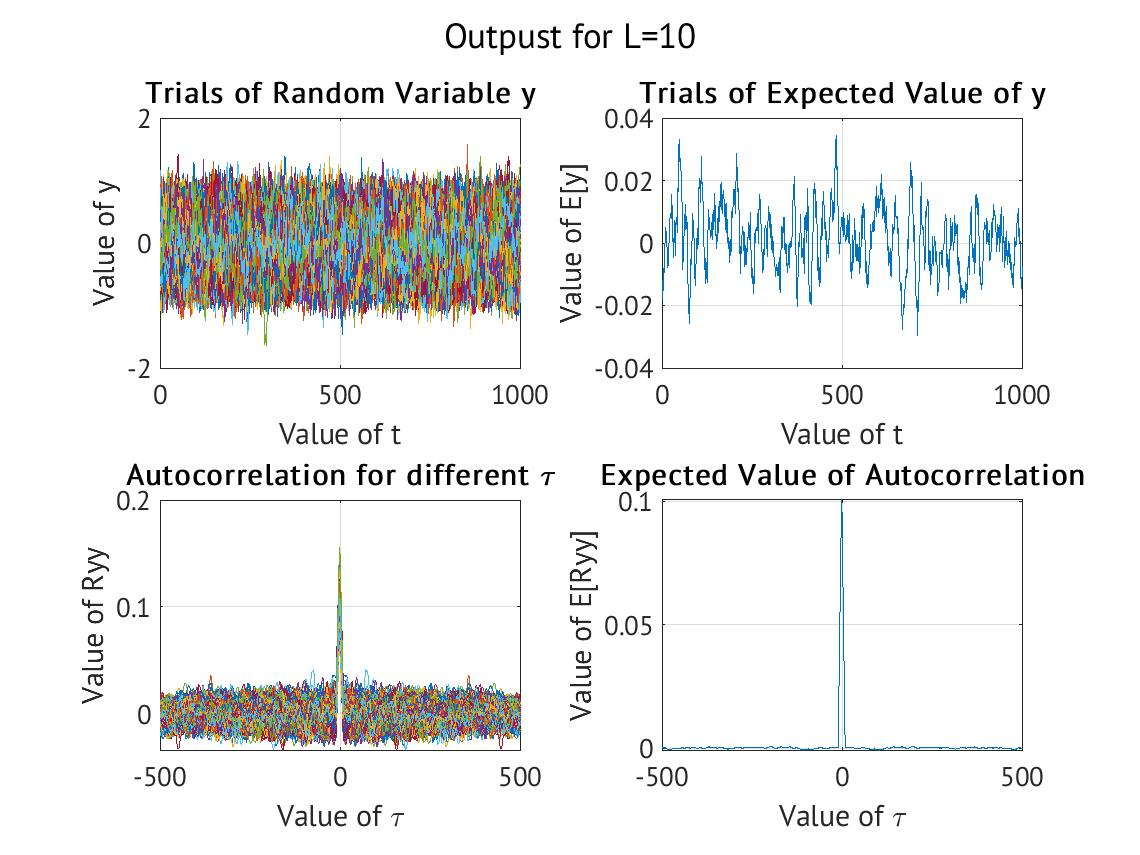
\includegraphics[width=.9\linewidth]{./Images/L10.jpg}
\caption{\label{fig:L10}Outputs of filtered random variable for L = 10}
\end{figure}

\begin{figure}[htbp]
\centering
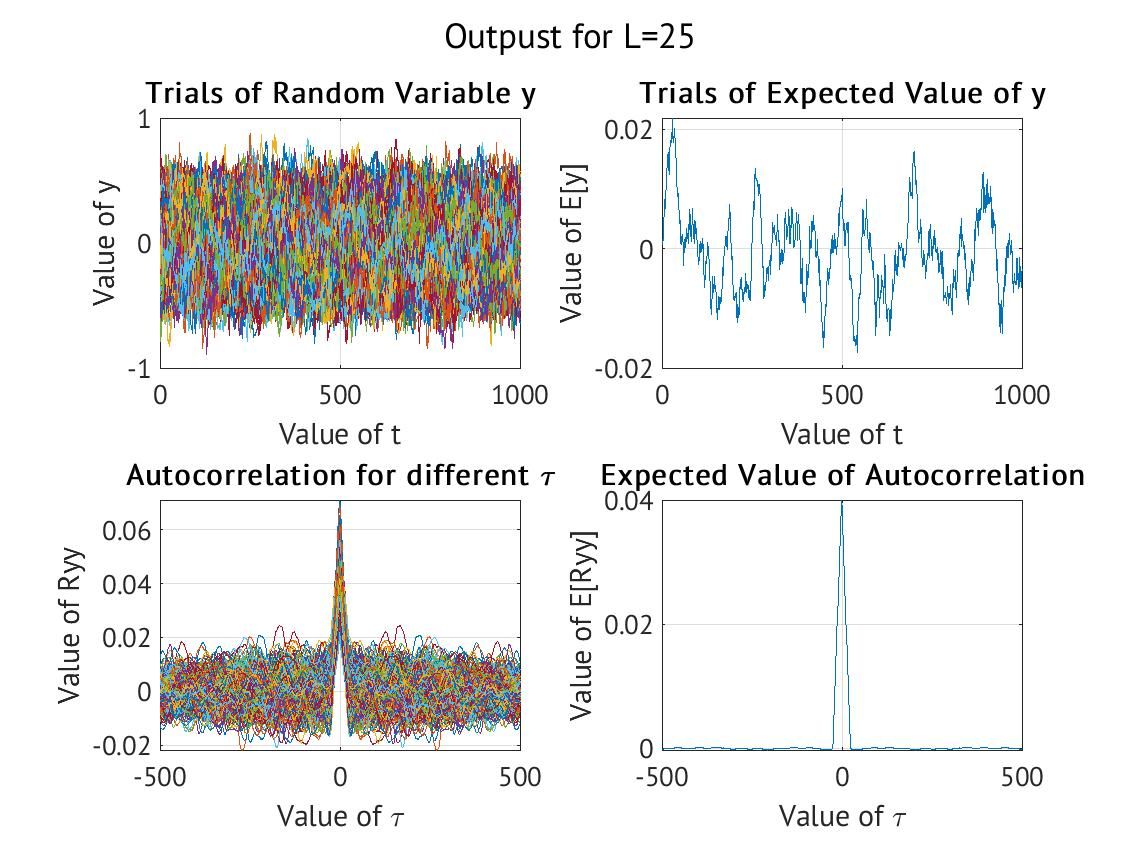
\includegraphics[width=.9\linewidth]{./Images/L25.jpg}
\caption{\label{fig:L25}Outputs of filtered random variable for L = 25}
\end{figure}

\begin{figure}[htbp]
\centering
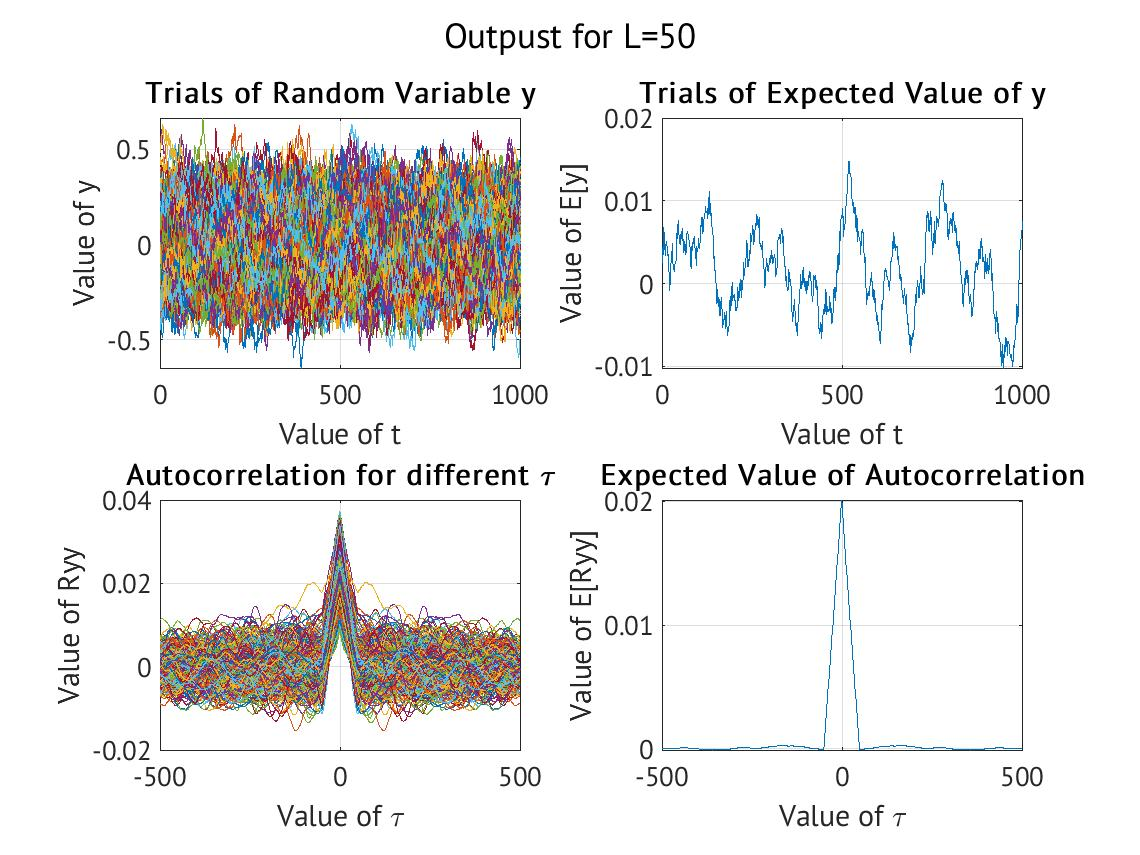
\includegraphics[width=.9\linewidth]{./Images/L50.jpg}
\caption{\label{fig:L50}Ouputs of filtered random variable for L = 50}
\end{figure}

\pagebreak
Each figure from above shows a very similar outcome that tracks intuition based on the inputs for each.
With each filter being applied to the random variables generated there is a trend that the max magnitude of the random variable shrinks. This is also reflected in the expected value of the random variable, which has a similar shrinking effect. The same was seen in Section \ref{sec:org375a5aa} as the expected value of a random variable is still random.

Similarly to Figure \ref{fig:MatlabModel} subfigure 3, each autocorrelation output has a similar form. That form being random until the values get nearest to \(\tau\) being 0. The largest difference that is seen is that instead of being 1, or nearly 1, value that spikes away from the randomness there are more and more values as L increases. This is explained as there is a greater amount of autocorrelation for values that are closer (and not just the same as in \(\tau = 0\)) due to the filtering smoothing out the random variable to be closer for any given time. As L increases, this output is much more noticable as not only does the spike widen, but the randomness trends to a higher autocorrelation the smaller that \(\tau\) ends up being, which is seen as the amplitude differences between \(\tau = \pm 500\) and those just outside the spike.

The expected value of the autocorrelation is supposed to be a delta function as stated earlier. Figures \ref{fig:L10}, \ref{fig:L25}, and \ref{fig:L50} are still close to this approximation, but with the difference of having a wider spike as there is a greater autocorrelation around those values of \(\tau\) as referenced above.

\medskip
These outputs show that as L increases the same trends hold, but to a differing degree of magnitude. In addition to this comparing the variance that is calculated from each trial is nearly equivalent to that of the value of L, as shown in Table \ref{tab:sigma} below.

\begin{table}[htbp]
\caption{\label{tab:sigma}Values of \(\sigma^2\) and \(g\) for each value of L}
\centering
\begin{tabular}{|c|c|c|c|}
\hline
L & 10 & 25 & 50\\
\(\sigma^2_y\) & 0.1003 & 0.0406 & 0.0201\\
\hline
\(\sigma^2_x\) & 0.9984 & 0.9984 & 0.9984\\
\hline
\(g\) & 9.9560 & 24.5676 & 49.6907\\
\hline
\end{tabular}
\end{table}

The value of \(g\) is calculated through \(g = \displaystyle\frac{\sigma^2_x}{\sigma^2_y}\), where \(\sigma^2_x\) is the variance calculated in Section \ref{sec:org375a5aa}, and \(\sigma^2_y\) is the newly calculated variance for each L. In doing this, \(g\) is found to approximate the value of L, which makes sense as the variance is dependent on L, thus dividing an unmodulated variance by a variance modulated by L yields L.

\section{What Was Learned}
\label{sec:org265fa1c}
This project teaches the process of autocorrelation and how to understand it in terms of random noise. The outputs that were generated in this show these effects through the random variables, though Section \ref{sec:orgb3c6090} has a greater effect on this understanding with the filtering affecting the output of the autocorrelation. The filtering makes the values more closely related and less random, which is then seen with the autocorrelation outputs where there is a larger \(\tau\) that autocorrelates. The topics learned in class were simplified and used in this project and the manipulation of the data aids in understanding these topics. Overall this project was a useful and good ending to the projects in this class.
\subsection{Changes}
\label{sec:org94474a1}
I personally feel that little to no changes are needed for this project. The topics are well documented in the lecture notes, as well as online if need be. On top of this is one of the more workable and simpler topics within the course so any issues can be ironed out quickly.

The process of working on this project took much less time than the others this semester, being only around 6-7 hours at the time of writing this.
\end{document}
